\documentclass{ujarticle}
\usepackage{ketpic,ketlayer}
\usepackage{amsmath,amssymb}
\usepackage{graphicx}
\usepackage{xcolor}
\usepackage{bm,enumerate}
\usepackage[dvipdfmx,colorlinks=true,urlcolor=blue]{hyperref}

\setmargin{15}{15}{15}{15}

\西暦

\renewcommand{\labelitemi}{・}
\pagestyle{empty}

\begin{document}

\begin{center}
KeTCindyを使うために
\end{center}

\vspace{-5mm}

\hfill 修正日:\today

\begin{enumerate}[\bf\large 1.]
\item Cinderella, R, Maxima とSumatra(Windowsのみ)をインストールする.\vspace{-2mm}

 \begin{itemize}
 \item \url{https://beta.cinderella.de}  (Cinderella)\\
\hspace*{6mm}注)Windowsの場合,保存してから右クリックして「管理者として実行」を選ぶ.
 \item \url{https://cran.r-project.org}   (R)
 \item \url{https://sourceforge.net/projects/maxima/files}  (Maxima)
 \item \url{https://www.sumatrapdfreader.org/download-free-pdf-viewer.html} (Sumatra)\\
\hspace*{6mm}注)Sumatraのインストール先は,オプションでProgram Files(またはx86)を指定する.

 \end{itemize}
\item TeXをインストールしていない場合はインストールする.\vspace{-2mm}
 \begin{enumerate}[(1)]
 \item TeXLiveを推奨 (2018以降ではketcindyが組み込まれている.ただし更新が必要)
 \item KeTTeXはTeXLiveの軽量版で以下からダウンロードできる.\\
\hspace*{3mm}\url{https://github.com/ketpic/kettex/releases}\\
    \hspace*{6mm}注)インストールの詳細は\verb|doc>readmemore|フォルダにあるReadmemore(Mac,Win)を参照.
%    \hspace*{5mm}注)Mac(Catalina)の場合,ターミナルで \verb|sudo spctl --master-enable| を実行
\end{enumerate}
 
\item KeTCindyのインストール(更新)\vspace{-2mm}
  \begin{enumerate}[(1)]
  \item ketcindyをCTAN(\url{https://ctan.org})からダウンロードする.
    \begin{itemize}

     \item ketcindyで検索 $>$ Package ketcindy $>$ {\color{red}Repository}」(最新版)
     \item Repositoryはgithubサイトにある{\color{red}最新版}へのリンク\\
        \hspace*{10mm}Code $>$ Download ZIP(フォルダ名はketcindy-master)
     \item \Ltab{8zw}{Windowsの場合}(i) {\color{red}OneDriveの管轄外で漢字や半角スペースが入らない場所(\verb|C:\|など)}に解凍する.\\
\Ltab{8zw}{}(ii) 解凍したら,{\color{red}ketcindy-masterをketcindyに名称変更しておく(\verb|-| 以降を削除)}
     \end{itemize}
\item docにある\verb|ketcindysettings.cdy|をダブルクリック(画面が狭ければ,右方向に広げる).
    \begin{itemize}
    \item 必要なら,実行プログラムをCinderellaに設定する.
    \item 他のcdyファイルを開いているときは,Cinderellaを一旦終了してからにする.

   \end{itemize}
  \item 画面上のボタン(1)(2)を選択して,(3)を順に実行する.
  \end{enumerate}

%\vspace{3mm}

\begin{layer}{140}{0}
\putnotese{17}{15}{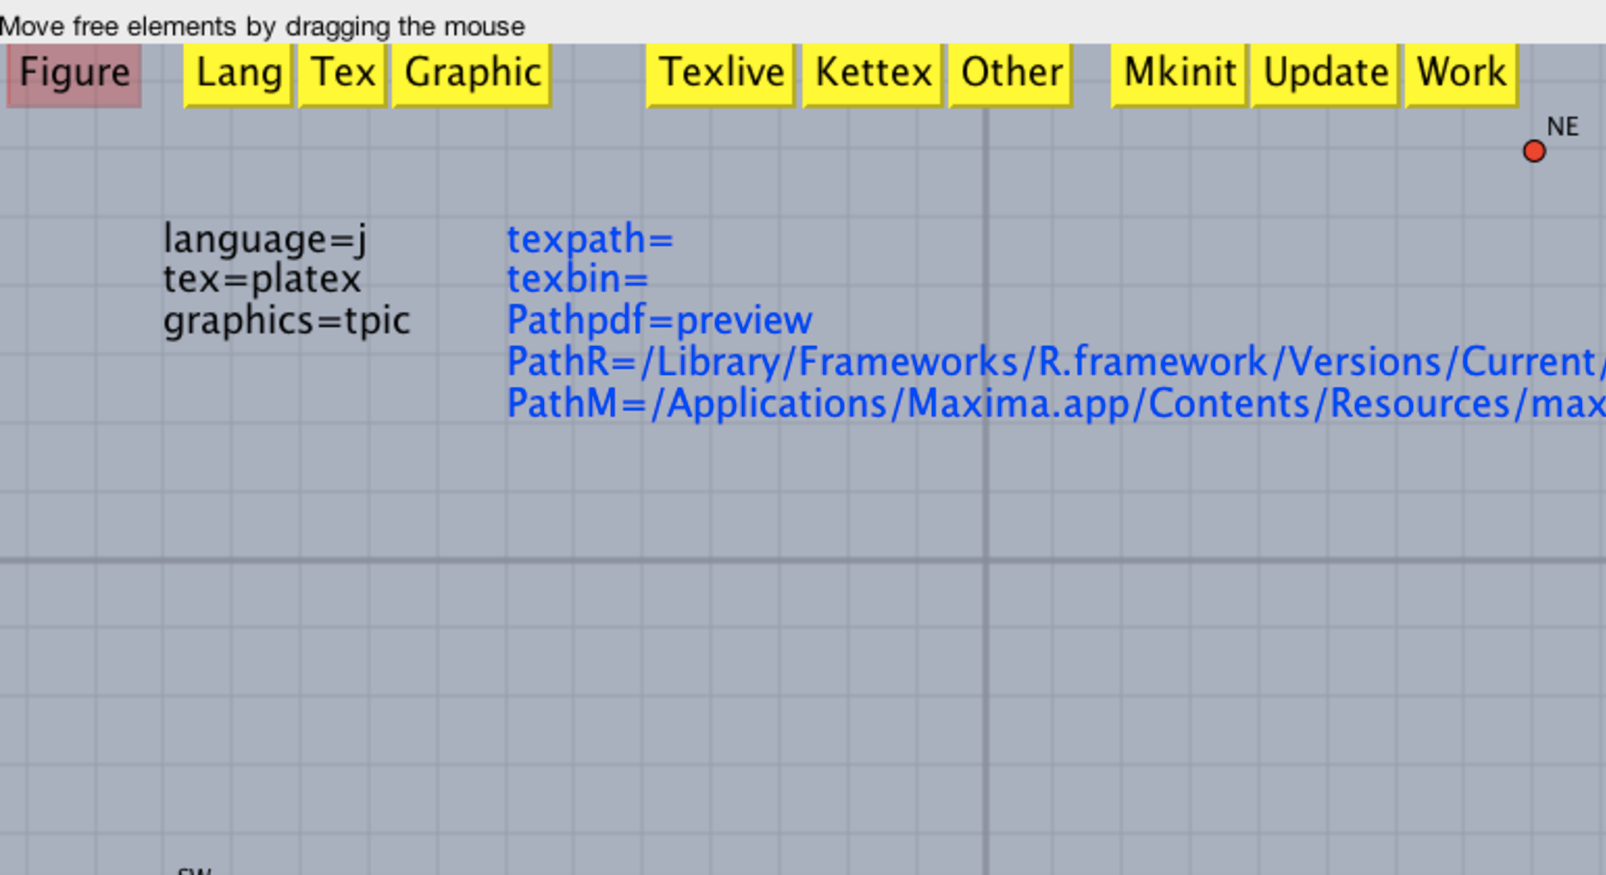
\includegraphics[bb=0.00 0.00 771.00 420.00,width=100mm]{Fig/setting.pdf}}
\putnotee{-10}{5}{\bf [1]\ 言語などの選択}
\putnotese{-7}{10}{\underline{Language}}
\putnotese{-5}{15}{\begin{tabular}{l}
Japanese\vspace{-1mm}\\English \end{tabular}}
\putnotese{-7}{25}{\underline{\TeX}}
\putnotese{-5}{29}{\begin{tabular}{l}
platex\vspace{-1mm}\\uplatex\vspace{-1mm}\\latex\vspace{-1mm}\\xelatex\vspace{-1mm}\\pdflatex\vspace{-1mm}\\lualatex\end{tabular}}
\putnotese{-7}{57}{\underline{Graphic Code}}
\putnotese{-5}{61}{\begin{tabular}{l}tpic\vspace{-1mm}\\pict2e\vspace{-1mm}\\tikz\end{tabular}}
\arrowline{34}{17}{18}{135}
\putnoten{73}{7}{\bf [2]\ \TeX システムの選択}
\arrowline{73}{17}{9}{90}
\putnotee{115}{5}{\bf [3]\ 作成と更新}
\arrowline{100}{17}{18}{45}
\putnotese{121}{9}{\fbox{Mkinit}}
\putnotese{123}{16}{\begin{minipage}[t]{52mm}%
初期設定ファイルketcindy.iniをユーザホーム(ホーム)に作成\\
%{\small 注)CinderellaのPluginsにおくとき\\
%\hspace*{3mm}CindyScript/ketlibの3行目を\\
%\hfill setdirectory(plugindirectory)にする}
\end{minipage}}
\putnotese{121}{30}{\fbox{Update}}
\putnotese{123}{37}{TeXシステムのketcindyを更新}
%\putnotese{126}{56}{実行時エラーの場合Helpを参照}
\putnotese{121}{47}{\fbox{Work}}
\putnotese{123}{54}{\begin{minipage}[t]{52mm}%
作業フォルダketcindy(+日付)をホームに作成
(samples, templates, manual)
\end{minipage}}
\end{layer}

\vspace{71mm}

\item テストラン\vspace{-2mm}

\begin{itemize}
 \item Cinderellaをいったん終了,ユーザホーム/ketcindy(+日付)/templtatesの1つのファイルをダブルクリック.
\item\verb|Figure|を押して,pdfが表示されれば成功
\end{itemize}

\item  その他\vspace{-2mm}
\begin{itemize}
\item \verb|ketcindy.ini|はデフォルトではユーザホームに作られる.\\
 ・\verb|CindyScripts>ketlib|の3行目を\verb|setdirectory(gethome());|とする.\\
 ・CinderellaのPluginsフォルダにコピーした場合は,\verb|setdirectory(plugindirectory);|とする.

\item エディタの設定などについては,\verb|doc>readmemore|フォルダにあるReadmemore(Mac,Win,Linux)を参照.
\end{itemize}
\end{enumerate}

\end{document}